\section{Gradual Permission Regions}

\begin{figure}[t]
  \centering
  \begin{lstlisting}
<T> void acquireR(T xs)
<T> void acquireR(T xs, int idx)
<T> void acquireR(T xs, int start, int end)

<T> void releaseR(T xs)
<T> void releaseR(T xs, int idx)
<T> void releaseR(T xs, int start, int end)
  \end{lstlisting}
\caption{The permission-region annotation interface for read acquisition and release in \jpf.}
\label{fig:pr-interface}
\end{figure}

\begin{figure}
  \begin{center}
    \begin{lstlisting}
public static void main(final String[] argv) {
  launchHabaneroApp(() -> {
    Stack stk = initStack();  

    finish(() -> {

      async(() -> {
        acquireW(stk);
        stk.push(5);
        releaseW(stk);
      });
      
      acquireR(stk);
      stk.peek();
      releaseR(stk);
    });
  });
}
\end{lstlisting}
  \end{center}
  \caption{The \hj\ program from \figref{fig:hj-async-finish} with additional permission region annotations.}
  \label{fig:hj-async-finish-pr}
\end{figure}

\begin{figure}[t]
\centering
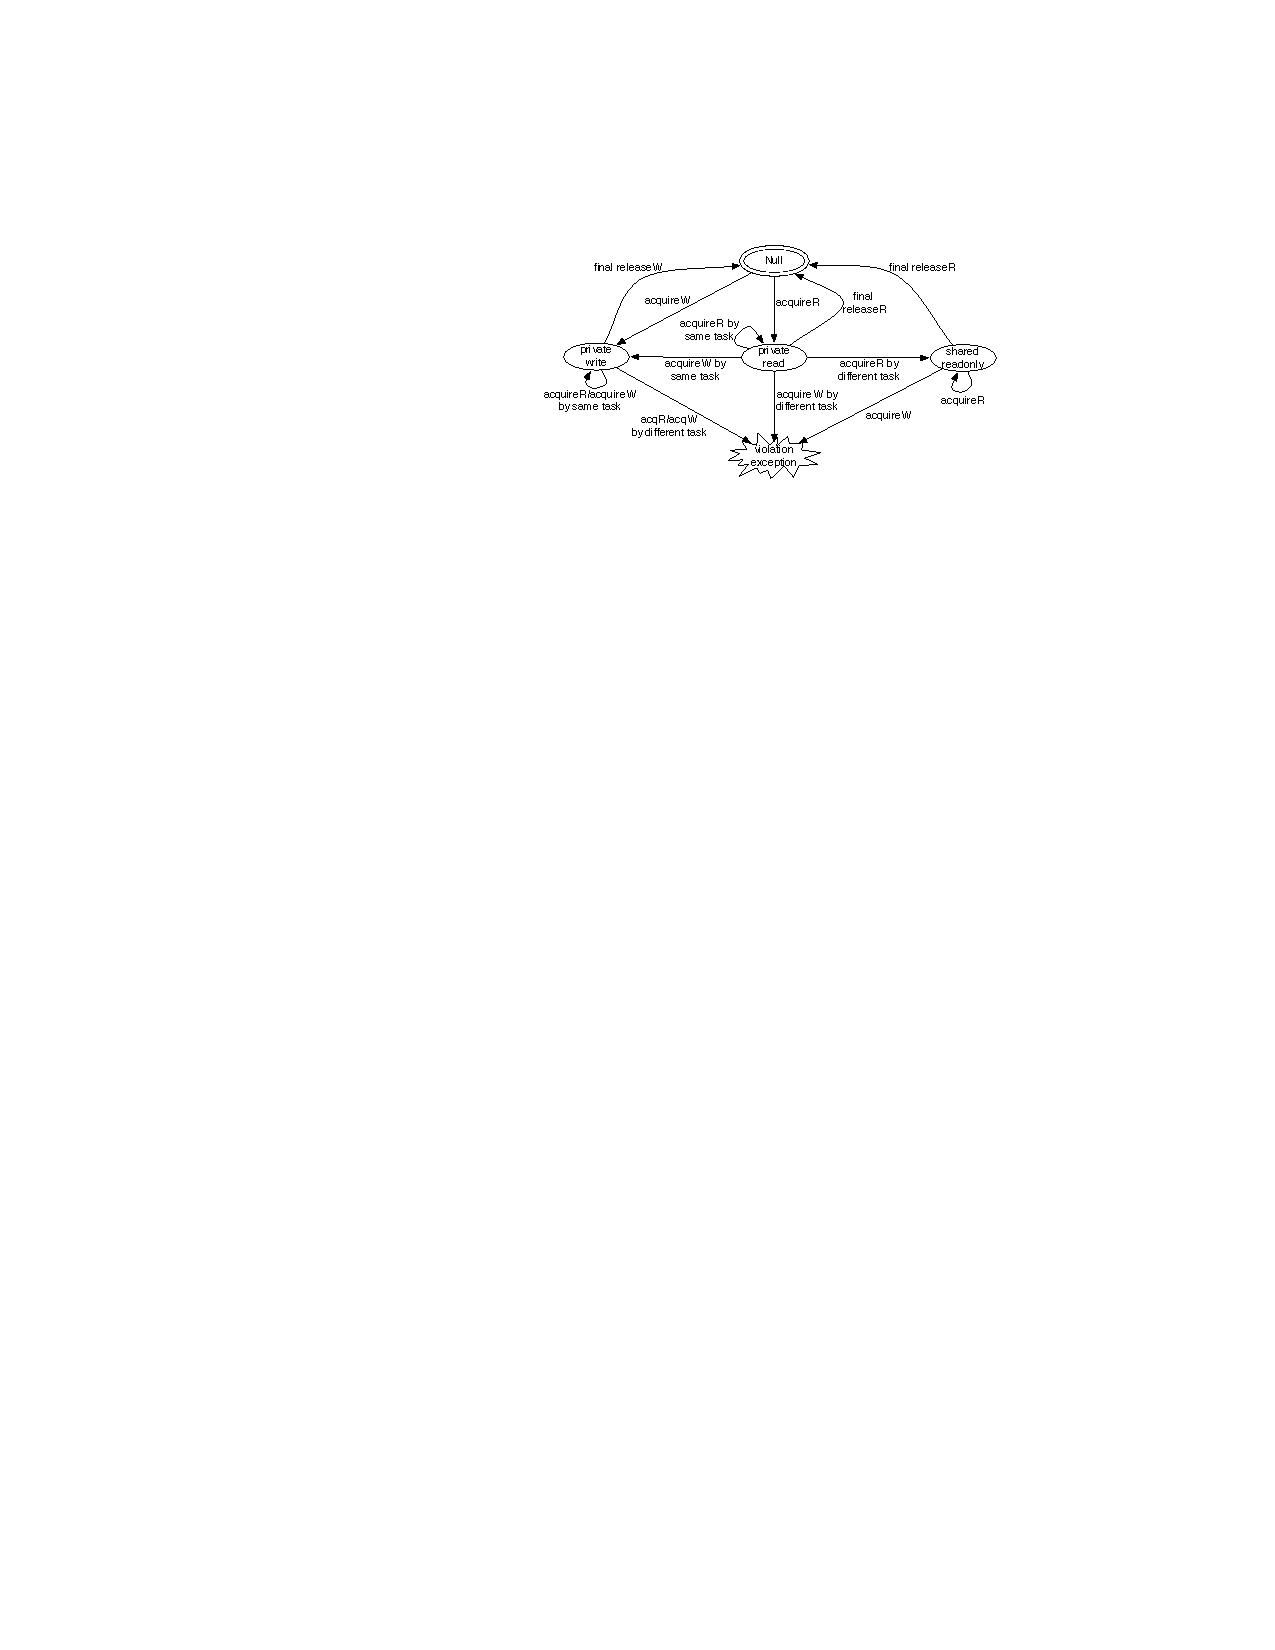
\includegraphics[width=3.25in]{../figs/state-machine}
\caption{State machine for permission regions operating on a single object.}
\label{fig:state-machine}
\end{figure}


\begin{figure}[t]
\centering
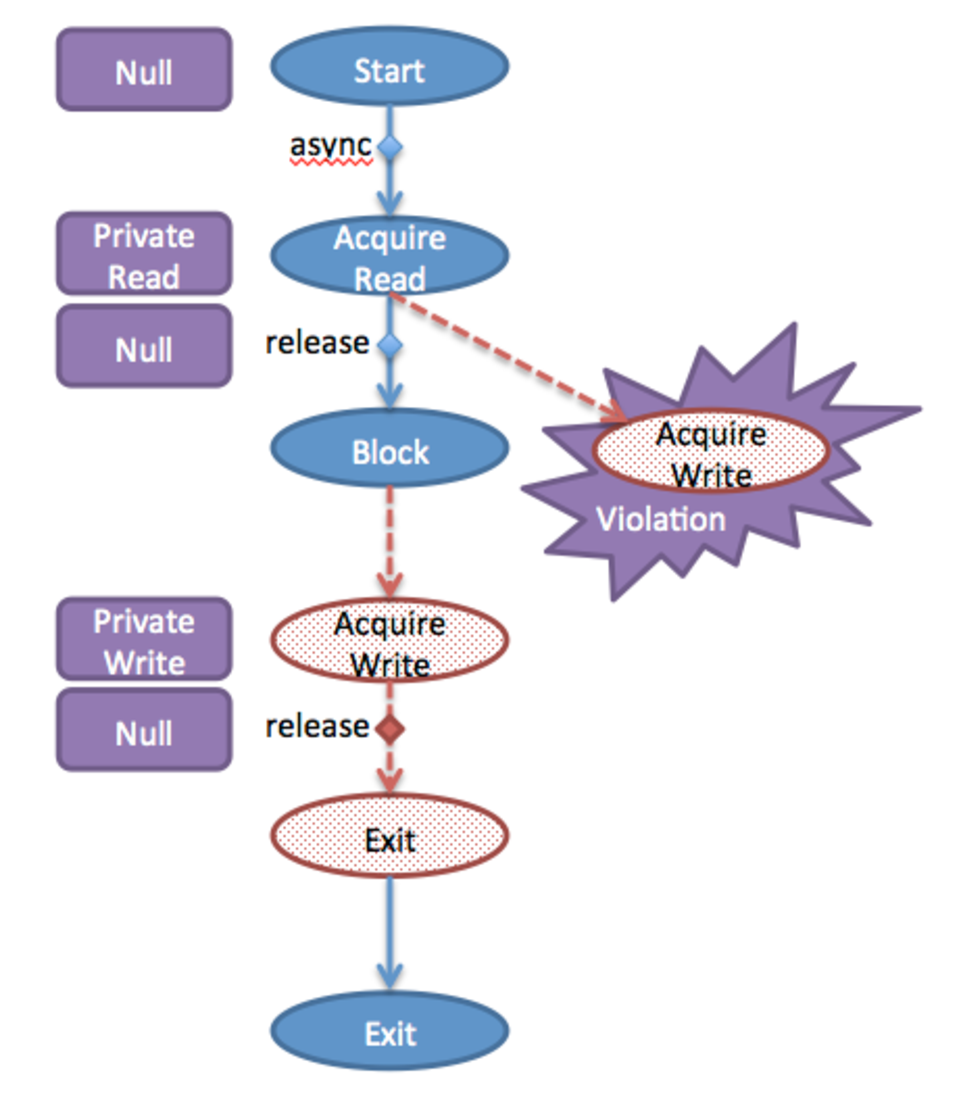
\includegraphics[width=3.25in]{../figs/stack-violation}
\caption{Different schedules for the program in \figref{fig:hj-async-finish} with the right-most schedule detecting a violation.}
\label{fig:permission-violation-state}
\end{figure}

Gradual permissions with permission regions is a hybrid
static-dynamic approach to detecting data-race in task-parallel
programs \cite{Westbrook:2011:PRR:2341616.2341627,hj-grad-perm}. The
programmer annotates regions of the program text that access shared
objects. Those regions are indicated as accessing shared objects in
read mode or write mode. When the program runs, a state machine is
associated with each shared object to track access permissions on that
object as indicated by the program annotations. If access permissions
from distinct tasks on the same object conflict, then a dynamic run-time
error is reported.

Permission regions are distinctly different from
\texttt{isolated}-constructs. Foremost, \texttt{isolated}-constructs define atomic regions that run mutually
exclusive to other regions in \texttt{isolated}-constructs. As such, isolation
restricts concurrency by serializing atomic regions. Permission regions
do not serialize atomic regions to restrict concurrency. They only
check if concurrent accesses to atomic regions are free of data-race. Isolation is
always best avoided given its impact on speedup in Amdahl's law.

Permission regions are annotated for \jpf\ using the interface in
\figref{fig:pr-interface}. Although the figure only shows the read
interface, the write interface follows the same pattern. The first method on the 
interface has arguments to manage permissions on a single object. The
second and third methods have arguments to manage permissions on
arrays. Arrays are somewhat more nuanced. Consider the following code:
\begin{lstlisting}
  f[i] = new C();
  f[i].write(j);
\end{lstlisting}
The first line writes to the array location $i$. The second line
writes to the object stored in the array location $i$. These two
accesses must be treated separately. As such, the permission regions interface provides
methods to manage permissions on a specific index in an array or a
range of indexes in the array. Permissions on the actual object in the array use the first method in the interface. The annotated code snippet from above is as follows.
\begin{lstlisting}
  acquireW(f,i);
  f[i] = new C();
  releaseW(f,i);
  
  acquireR(f,i);
  acquireW(f[i]);
  f[i].write(j);
  releaseW(f[i]);
  releaseR(f,i);
\end{lstlisting}

\figref{fig:hj-async-finish-pr} is the permission-region annotated
version of the program in \figref{fig:hj-async-finish} from the
previous section. The operations on the shared object \texttt{stk} are
now wrapped in calls to acquire or release permissions on the shared
object. Note that the permission regions span all the code 
in the \texttt{stk.push} and \texttt{stk.peek} methods, so anytime the object is referenced, it is covered. In this
way, permission regions can be as large or as small as desired. If the
regions are too large, however, then the approach may report a data-race
where no race exists
\cite{Westbrook:2011:PRR:2341616.2341627,hj-grad-perm}. 

\figref{fig:permission-violation-state} is the state-machine to track
permissions on shared objects and detect violations. That machine is included here for convenience directly
from \cite{hj-grad-perm}. The machine starts in the double-circled
\textit{Null} state. On acquisition or release, the machine updates to
the appropriate state based on its current state. The machine signals
a violation if it ever detects conflicting accesses by different tasks.

\figref{fig:permission-violation-state} shows two possible schedules
for the annotated program in \figref{fig:hj-async-finish-pr}. The solid
filled ovals and solid lines represent the main task and the dotted
filled ovals and dashed lines represent the task created by the
\texttt{async}-statement. The squares indicate the current state of
the state machine that is tracking accesses to the shared object
\texttt{stk}.

The left branch of the tree is the schedule where the main task runs
until it is blocked by the \texttt{finish}-statement where it must
join with the tasked created by the \texttt{async}-statement. The main
task acquires and releases private read privileges on the region
before it blocks. After the main task blocks, the newly created task
runs, acquiring and releasing private write privileges, and it then
exits. If this schedule is followed in the run-time, then no
violation is reported even through data-race exists in the
program. The approach is run-time dependent and not exhaustive.

The right branch is an alternate schedule that is possible in the
program. In this schedule, the newly created task from the
\texttt{async}-statement runs just after the main task acquires private
read privileges on the shared object. When the new task tries to
acquire write privileges, the state-machine that manages permissions on
the shared object moves into the violation state to report the error.

\subsection{Permission Regions in \jpf}

The implementation of permission regions in \jpf\ spans 1036
lines of code and covers 11 distinct class objects. It leverages
\jpf's ability to track thread IDs of all accesses to objects, so it not only reports
violations on the permission regions, but also identifies shared
accesses that are not annotated by permission regions or covered by \texttt{isolated}-constructs. In this way,
\jpf\ updates the user when a shared access has been missed in the
annotations.

The implementation uses two key features of \jpf: byte-code listeners
and object attributes. It installs a byte-code listener to watch for
instances of the \texttt{INVOKE}-code. The actual methods for the permission regions interface in
\figref{fig:pr-interface} are empty stubs. When
the listener sees an instance of the \texttt{INVOKE}-code that calls a
method on the interface, it gets the method's parameters from
the stack and updates the associated state-machines appropriately.

The state machines themselves reside in an attribute of the object. Every object
in \jpf\ has an associated attribute that can hold arbitrary information. For
example, attributes are used to implement symbolic execution in \jpf\
\cite{DBLP:journals/ase/PasareanuVBGMR13}. The important property of attributes
is that they follow heap objects through the entirety of state space
exploration. The state machines to track permission region accesses are stored
in those attributes. For arrays, a separate permissions state-machine is stored
for every index. The program annotations acquire and release permissions on
individual indexes (or a range of indexes) as mentioned previously.

With or without permission regions, \jpf\ finds the data-race in
\figref{fig:hj-async-finish-pr} using its built-in precise-data-race
listener with \hjv. Unfortunately, \jpf\ times-out on larger programs due to
state-explosion as shown in the results section. Permission regions
are utilized to improve this limitation.
